% =============================================================================
% File:  intro_git.tex -- Introduction to Git 
%
% =============================================================================

\documentclass[10pt,xcolor=dvipsnames]{beamer}

\usetheme{Madrid}

%\renewcommand\mathfamilydefault{\rmdefault}
\usefonttheme[onlymath]{serif}

%\usecolortheme{seahorse}
\usepackage[utf8]{inputenc}
\usepackage{xcolor}
\usepackage{colortbl}
\usepackage{verbatim}
%gets rid of bottom navigation bars
\setbeamertemplate{footline}{}
%gets rid of navigation symbols
\setbeamertemplate{navigation symbols}{}
%\usetheme{Frankfurt}
%\usetheme{Rochester}
%\usepackage{beamerthemeshadow}

% \usepackage{amsmath}
% \usepackage{amssymb}

%\usepackage{floatflt}
%\usepackage[utf8]{inputenc}
%\usepackage{multirow}
    \usepackage{mathptmx}
\graphicspath{{./pics/}{./figs/}}
\usepackage{graphicx}          % Include this line if your 
                               % document contains figures,
\usepackage[super]{nth}
\usepackage{multirow}
\usepackage{amsmath}
\usepackage{verbatim}




%%%%%%%%%% Header %%%%%%%%%%%%
\title{Short Introduction to Git}
\subtitle{Grup Seminar}

\author{Andr\'as Hartmann, Sascha Zickenrott}
\institute[LCSB]{
LCSB, Computational Biology group
  University of Luxembourg
}
% Mandatory to **declare** a logo to be placed on the bottom right -- normally the
% university logo. ADAPT ACCORDINGLY:

\date[June 29, 2016]{June 29, 2016, Luxembourg}

\logo{
\includegraphics[height=0.10\paperheight]{logo_UL.pdf} \hspace{0.2in}\vspace{0.2in}}

%%%%%%%%%%%%% Body %%%%%%%%%%%%%%%
\begin{document}

\begin{frame}
  \vspace{2.5em}
\begin{center}
    
\includegraphics[height=0.2\textheight]{git-logo.jpg}
\end{center}
  \titlepage
\end{frame}

\section{Introduction}

\begin{frame}{Why VCS?}{Version Control Systems}
Do you remember this?\\
\centering
    
\includegraphics[height=0.8\textheight]{Finaldoc.png}
\end{frame}

\begin{frame}{Why VCS?}{Version Control Systems}
And this?\\
\centering
    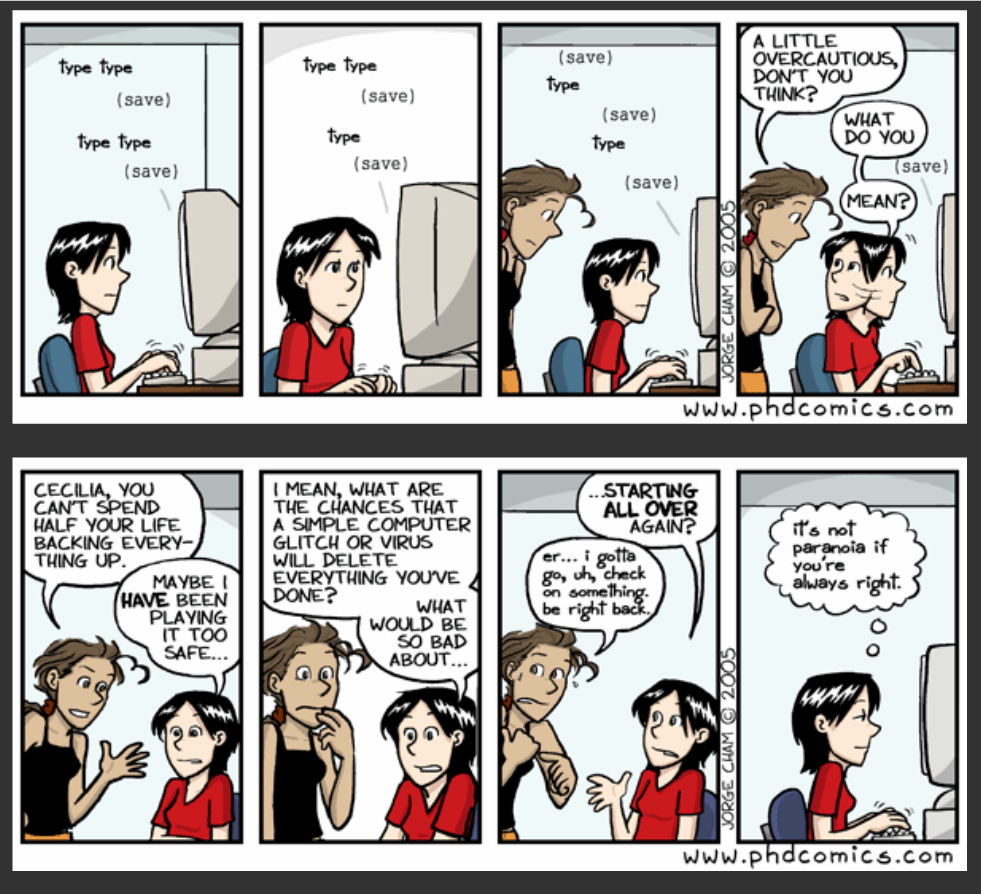
\includegraphics[height=0.8\textheight]{ctrl-s.png}
\end{frame}

\begin{frame}{Why VCS?}{Version Control Systems}
\begin{itemize}
  \setlength\itemsep{0.2in}
\item Storing versioned files on the easy way
\item Collaboration
	\begin{itemize}
	\item Sharing files
	\item Collaborative editing
	\item Review changes, trace problems
	\item Optimal team work-flow
	\end{itemize}
\item Backup \& History
	\begin{itemize}
	\item Ultimate ctrl-z
	\item Remote / local storage
	\item Logs: Forced comments to all revisions
	\end{itemize}
\end{itemize}
\end{frame}

\begin{frame}{What kind of data?}{Version Control Systems}
\begin{itemize}
  \setlength\itemsep{0.4in}
\item Mainly {\bf text} files\\
- Source code, txt files, \LaTeX\  source, etc ...
\item No sophisticated difference for binary files\\
- Word, Excel documents, pictures, pdfs ...
\item For \LaTeX\ collaborative editing you may want to try\\
- sharelatex: https://www.sharelatex.com
\end{itemize}
\end{frame}



\begin{frame}{Why git?}
\begin{itemize}
\item{Distributed}
\end{itemize}
\end{frame}

\section{Start using GIT}
\begin{frame}{Further reading}
\begin{itemize}
\item{Distributed}
\end{itemize}
\end{frame}


\end{document}

